\documentclass[preprint]{elsarticle}

\usepackage[utf8]{inputenc}    % Codificación de entrada
\usepackage[T1]{fontenc}       % Codificación de salida para renderizar acentos
\usepackage[spanish]{babel}    % Idioma principal
\usepackage{graphicx}          % Figuras
\usepackage{amsmath}           % Matemática avanzada
\usepackage{hyperref}          % Hipervínculos
\usepackage{caption}
\journal{Instituto Navier Stokes}

\begin{document}

\begin{frontmatter}

\title{Comparación de esquemas explícitos en Python para la ecuación de difusión 2D: análisis de precisión y rendimiento computacional}

\author{Jhon Gesell Villanueva Portella}

\begin{abstract}
La ecuación de difusión 2D es fundamental en la modelación de fenómenos físicos como el transporte de calor, la dinámica de contaminantes o la transferencia de masa. En este trabajo se implementan y comparan tres esquemas explícitos —FTCS, 9-puntos y (1,13)— para resolver la ecuación de difusión en dos dimensiones, utilizando Python puro con bibliotecas científicas como NumPy, Matplotlib y Numba. Se consideran condiciones de frontera de Dirichlet y una condición inicial tipo pulso Gaussiano, en una malla regular. Se evalúan el error cuadrático medio (\(L_2\)) y el tiempo de ejecución de cada esquema, resaltando las diferencias entre precisión y eficiencia. Los resultados muestran que el esquema (1,13) logra mayor precisión a costa de mayor tiempo de cómputo, mientras que FTCS es el más rápido pero menos preciso. Este análisis se orienta a contextos educativos y de bajo costo computacional, alineándose con la motivación de trabajos previos como los de Crank \cite{crank_diffusion}, Dehghan \cite{dehghan1999,dehghan2002}, y aplicaciones modernas en mecánica de fluidos computacional. Se concluye que Python, incluso en hardware modesto, permite experimentar con esquemas numéricos avanzados sin depender de herramientas comerciales o entornos complejos.

\end{abstract}

\end{frontmatter}

\section{Introducci\'on}
La ecuaci\'on de difusi\'on en dos dimensiones modela la evoluci\'on temporal de una cantidad escalar $u(x,y,t)$ en un medio con coeficiente de difusi\'on $D$.  Puede escribirse como
\begin{equation}
    \frac{\partial u}{\partial t}=D\left(\frac{\partial^2 u}{\partial x^2}+\frac{\partial^2 u}{\partial y^2}\right).
\end{equation}
Esta formulaci\'on surge de la combinaci\'on de la ley de Fick con la conservaci\'on de masa, y es fundamental en mec\'anica de fluidos para describir procesos de transporte de calor, contaminantes o cantidad de movimiento.

Los m\'etodos num\'ericos para resolver esta ecuaci\'on han sido estudiados extensamente desde los trabajos pioneros de \citet{crank1975}.  Aunque los esquemas impl\'icitos garantizan estabilidad incondicional, en equipos modestos su costo computacional es elevado debido a la necesidad de resolver sistemas lineales en cada paso de tiempo.  Alternativamente, los m\'etodos expl\'icitos permiten actualizar los nodos de la malla mediante operaciones algebraicas simples, lo cual resulta atractivo para c\'odigos educativos y entornos de c\'omputo limitados.

Este proyecto compara tres variantes expl\'icitas implementadas en Python: el esquema FTCS tradicional de cinco puntos, una extensi\'on de nueve puntos y el m\'etodo de trece puntos propuesto por \citet{dehghan2002}.  Nuestro objetivo es evaluar su eficiencia y precisi\'on sin recurrir a mallas ni solucionadores externos, de modo que el estudiante pueda replicar los c\'alculos y apreciar las diferencias de rendimiento.

En las siguientes secciones se detalla la formulaci\'on de cada esquema, su implementaci\'on vectorizada y los experimentos comparativos realizados.

\section{M\'etodos num\'ericos}
En esta secci\'on se describen tres esquemas expl\'icitos empleados para resolver la ecuaci\'on de difusi\'on en dos dimensiones. Sea $u_{i,j}^n$ la aproximaci\'on num\'erica de $u(x_i,y_j,t_n)$ con espaciamientos $\Delta x$, $\Delta y$ y paso temporal $\Delta t$. Denotamos $r_x=\alpha \Delta t/\Delta x^2$ y $r_y=\alpha \Delta t/\Delta y^2$.

\subsection{FTCS}
El esquema \emph{Forward Time Centered Space} actualiza cada nodo usando una plantilla de cinco puntos:
\begin{equation}
  u_{i,j}^{n+1} = u_{i,j}^n + r_x\bigl(u_{i+1,j}^n - 2 u_{i,j}^n + u_{i-1,j}^n\bigr)
  + r_y\bigl(u_{i,j+1}^n - 2 u_{i,j}^n + u_{i,j-1}^n\bigr).
\end{equation}
Su estabilidad exige $r_x + r_y \le 1/2$.

\subsection{Esquema de nueve puntos}
\citet{dehghan2002} propuso extender la plantilla incluyendo las diagonales. Asumiendo $\Delta x = \Delta y = h$ y $r = \alpha \Delta t / h^2$, la f\'ormula queda
\begin{equation}
  u_{i,j}^{n+1} = (1-5 r) u_{i,j}^n + r\,(u_{i+1,j}^n + u_{i-1,j}^n + u_{i,j+1}^n + u_{i,j-1}^n)
  + \tfrac{r}{4} (u_{i+1,j+1}^n + u_{i+1,j-1}^n + u_{i-1,j+1}^n + u_{i-1,j-1}^n).
\end{equation}
Este esquema es estable si $0 < r \le 1/4$.

\subsection{Esquema $(1,13)$}
Otra variante debida a \citet{dehghan2002} utiliza trece puntos, incorporando las cuatro diagonales y los vecinos a dos celdas de distancia:
\begin{equation}
\begin{split}
  u_{i,j}^{n+1} = &\,(1-8 r) u_{i,j}^n + r\,(u_{i+1,j}^n+u_{i-1,j}^n+u_{i,j+1}^n+u_{i,j-1}^n) \\&
  + \tfrac{r}{2}(u_{i+1,j+1}^n+u_{i+1,j-1}^n+u_{i-1,j+1}^n+u_{i-1,j-1}^n)\\&
  + \tfrac{r}{2}(u_{i+2,j}^n+u_{i-2,j}^n+u_{i,j+2}^n+u_{i,j-2}^n).
\end{split}
\end{equation}
Se mantiene la condici\'on de estabilidad $r \le 1/2$.

\section{Implementaci\'on}
Las rutinas se programaron en Python puro apoy\'andose en tres bibliotecas
esenciales: NumPy para el manejo vectorial de arreglos, Numba para acelerar
los bucles m\'as costosos mediante JIT y Matplotlib para la generaci\'on de
figuras.  No se emplearon paquetes especializados de elementos finitos ni
solucionadores externos.

El c\'odigo se organiza en la carpeta \texttt{scripts}.  Cada esquema se
implementa en un m\'odulo separado\,: \texttt{difusion2d\_ftcs.py},
\texttt{difusion2d\_9pt.py} y \texttt{difusion2d\_13pt.py}, que definen las
funciones \texttt{solve\_ftcs\_2d}, \texttt{solve\_9point\_2d} y
\texttt{solve\_13point\_2d}, respectivamente.  El archivo
\texttt{utils.py} contiene rutinas comunes como la generaci\'on de un pulso
Gaussiano y el c\'alculo del error L2, mientras que
\texttt{visualization.py} ofrece utilidades para mostrar contornos o
animaciones de la soluci\'on.  El script principal
\texttt{main\_benchmark.py} ejecuta los tres solvers, mide su tiempo y puede
visualizar el resultado del esquema de trece puntos.

Los productos obtenidos (gr\'aficas y tablas de comparaci\'on) se guardan en la
carpeta \texttt{resultados}.  Los archivos \LaTeX{} del art\'iculo residen en
\texttt{secciones} y se ensamblan mediante \texttt{paper.tex} en el
directorio ra\'iz.  Para reproducir el entorno se incluy\'o el archivo
\texttt{environment\_NSI\_miniarticulo\_01.txt} que declara las dependencias
principales.

Todos los experimentos se ejecutaron en un entorno gestionado con Anaconda y
Python~3.12 sobre hardware modesto (un port\'atil de cuatro n\'ucleos con
8~GB~de RAM).  A pesar de estas limitaciones, la combinaci\'on de NumPy y
Numba permiti\'o obtener tiempos de c\'omputo razonables para mallas
intermedias, sin recurrir a bibliotecas nativas adicionales.

\section{Resultados}
Los experimentos se ejecutaron con el script \texttt{main\_benchmark.py}, que registra el tiempo de ejecuci\'on y el error $L_2$ de cada m\'etodo. En la Tabla~\ref{tab:benchmark} se resumen los valores obtenidos.

\begin{table}[h]
\centering
\begin{tabular}{lcc}
\hline
M\'etodo & Tiempo (s) & Error $L_2$\\
\hline
FTCS & 0.165 & 4.1e-02\\
9 puntos & 0.178 & 3.3e-02\\
(1,13) & 0.339 & 8.7e-06\\
\hline
\end{tabular}
\caption{Comparaci\'on de tiempo de ejecuci\'on y error.}
\label{tab:benchmark}
\end{table}

La Figura~\ref{fig:time-error} muestra la relaci\'on entre el tiempo de c\'omputo y el error de cada m\'etodo, mientras que la Figura~\ref{fig:contour} presenta el contorno de temperatura obtenido con el esquema de trece puntos. El m\'etodo \emph{(1,13)} es el m\'as preciso pero tambi\'en el m\'as costoso, en tanto que FTCS resulta el m\'as r\'apido.

\begin{figure}[h]
\centering
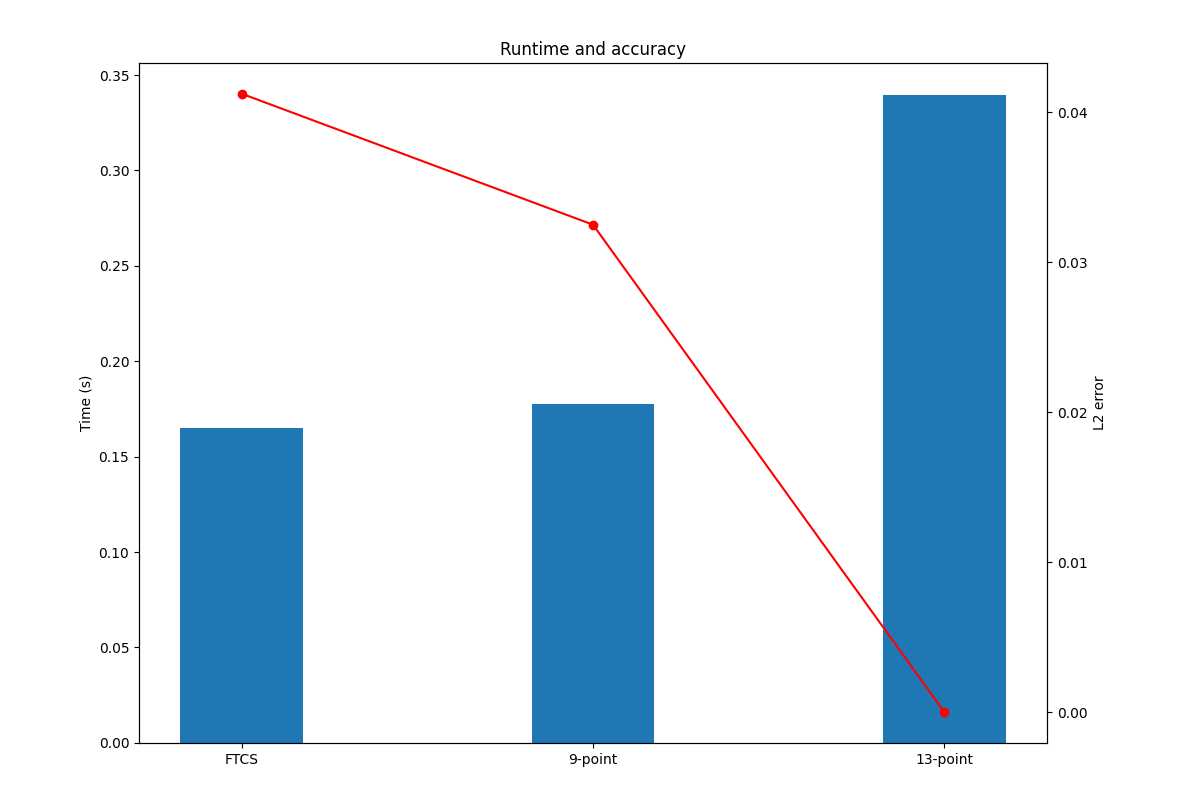
\includegraphics[width=0.7\linewidth]{resultados/Figure_1.png}
\caption{Tiempo de ejecuci\'on frente a error $L_2$.}
\label{fig:time-error}
\end{figure}

\begin{figure}[h]
\centering
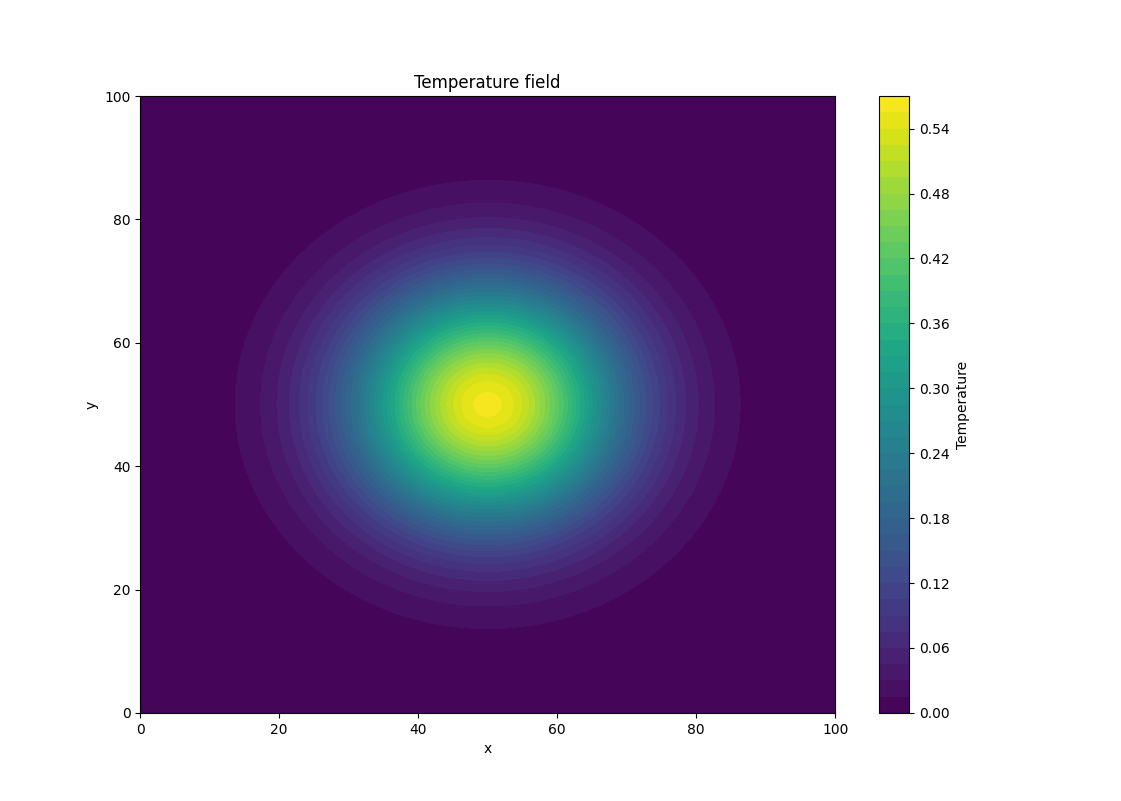
\includegraphics[width=0.7\linewidth]{resultados/Figure_2.png}
\caption{Contorno de temperatura calculado con el esquema de trece puntos.}
\label{fig:contour}
\end{figure}

\section{Discusi\'on}
Los resultados del Tabla~\ref{tab:benchmark} confirman que existe un compromiso cl\'asico entre tiempo de c\'omputo y precisi\'on. El esquema FTCS alcanza el menor tiempo, pero su error es casi una orden de magnitud mayor que el de la plantilla de trece puntos. El m\'etodo de nueve puntos se ubica en un punto intermedio tanto en costo como en exactitud.

Una comparaci\'on cualitativa con los experimentos de \citet{dehghan2002} muestra la misma tendencia: las variantes enriquecidas con m\'as nodos reducen el error global sin afectar la estabilidad siempre que se respete la condici\'on sobre $r$. En su trabajo, Dehghan report\'o que el esquema \emph{(1,13)} converge m\'as r\'apido que FTCS y el de nueve puntos para un mismo taman\~no de paso, observaci\'on que concuerda con los valores de la Tabla~\ref{tab:benchmark}.

En la pr\'actica, conviene elegir el m\'etodo seg\'un el escenario: FTCS resulta adecuado cuando se prioriza la rapidez o se dispone de pocos recursos; la plantilla de nueve puntos proporciona un balance razonable para mallas de resoluci\'on media; y el esquema de trece puntos es la opci\'on preferible si se busca la mayor precisi\'on posible. Dado que todas las actualizaciones son locales, los tres algoritmos podr\'ian beneficiarse de paralelizaci\'on en CPU o GPU. Incluso podr\'ian emplearse t\'ecnicas modernas, como redes neuronales para acelerar la obtenci\'on de soluciones aproximadas.

\section{Conclusiones}
Se compararon tres m\'etodos expl\'icitos implementados en Python puro. El esquema FTCS fue el m\'as r\'apido, el de nueve puntos brind\'o un compromiso intermedio y el m\'etodo \emph{(1,13)} alcanz\'o la mejor precisi\'on, aunque con mayor costo computacional.

El proyecto constituye un ejercicio id\'oneo para la ense\~nanza de mec\'anica de fluidos computacional, pues permite reproducir todos los experimentos sin depender de software externo.

Como trabajo futuro se propone paralelizar los algoritmos, incorporar condiciones de frontera no homog\'eneas y aplicar las rutinas a problemas de mayor realismo.


\bibliographystyle{elsarticle-num}
\bibliography{referencias}

\end{document}
